\chapter{Method}
This chapter describes the different steps of implementing the automatic package measuring algorithm.
The tools, components, and algorithms used are described.
Finally, the method used to evaluate the outcome are described.

\section{Implementation} \label{method:implementation}
This section presents how the package measuring solution was implemented.
First, the image processing tools used, and the process of detecting the reference object and package is described.
Then, the process of calculating the dimensions of the package, using the theory presented in chapter \ref{chapter:projective_geometry} and the detected object points, is described.

\subsection{OpenCV}
The most important tool used in this thesis is the library OpenCV.
It is used extensively in this thesis, and therefore deserves an introduction.

OpenCV is an open source library for computer vision.
It contains over 2500 optimised, state-of-the-art computer vision algorithms \cite{opencv_about}.
The functions in OpenCV range from low-level image filters to high-level algorithms for object recognition, camera calibration, pose estimation, machine learning, and much more.

OpenCV has a large community backing it, consisting of both startup companies, large corporations and researchers.
Development is led by the Russian company Itseez, and among the supporters are Google, Microsoft, Intel, IBM and Toyota \cite{opencv_about}. 

OpenCV is written in C++, but also has full interfaces for Python, Java and MATLAB and supports a variety of platforms, including Windows OS X, Linux, Android and iOS \cite{opencv_about}.
The native C++ interface was used in this thesis.

\subsection{Image processing}
One of the goals in image processing is to subjectively improve the quality of an image. 
The image is typically a digital image, swhich consists of small image elements, pixels.
Running image processing algorithms are often the first steps in computer vision systems, which is often referred to as preprocessing.
Both the input and output of an image processing algorithm are typically images, for example algorithms for noise reduction, contrast enhancement, and colour correction \cite[p. 1-2]{gonzalez-woods}. 

As the purpose is subjective improvement of quality, the means of performing preprocessing varies greatly depending on the application.
In this case, the aim is to reduce noise, and to remove irrelevant information from the image.
This is accomplished by converting the colour image to a grayscale image, followed by applying a median filter. 
A median filter was chosen because it reduces noise effectively, while also removing small, unwanted features from the image, such as small labels and marks on the package or the rest of the scene.
At the same time edges are preserved.
As the name implies, the median filter assigns the value of every pixel to the median of itself, and the neighbouring pixels within a certain radius \cite{huang1979fast}.

\subsection{Edge detection}
After preprocessing, the next step was to extract features from the image which can be used to make an interpretation of the image.
More specifically, the features that were extracted are edges. 
This was done using Canny's edge detection algorithm \cite{canny}. % TODO some additional comment maybe?
The outline of Canny's algorithm is as follows:
\begin{enumerate}
	\item Apply a smoothing image filter to reduce noise. A Gaussian filter is typically used, but a median filter was found to work better for this application.
	\item Find the intensity gradient of the image, i.e. the first derivative of the intensity along the x-axis and y-axis combined. The result is an image which is bright where the intensity changes rapidly, i.e. there is an edge.
	\item Apply non-maximum suppression, which is an edge thinning technique. The gradient image can often be blurry and contain thick edges. Non-maximum suppression on only keeps the local maxima, and sets the rest of the values to 0.
	\item Hysteresis, to remove false edges. At this point, the intensity image will contain many weak edges which are irrelevant. To remedy this, two thresholds are used, a low threshold and a high threshold. Pixels in the gradient image with a value lower than the low threshold are rejected, and pixels with a value  higher than the high threshold are accepted. Pixels with values in between the two thresholds are accepted if they are connected to a pixel above the high threshold. Accepted pixels are set to 1, and rejected pixels to 0, resulting in an accurate, binary edge image.
\end{enumerate}

% TODO skriva något om contour analysis?  \cite{suzuki}
%
\subsection{Line detection} %TODO tempus korrekt? % TODO add image? of sinusoids and each step.
Since the package consists of a set of lines, and and the edge image is difficult to interpret as it is, it seems like a good idea to find the lines in the image.
This was done with the Hough transform \cite{illingworth1988survey}.
The Hough transform can be used to detect many shapes.
The idea behind the Hough transform for line detection is as follows:
\begin{enumerate}
	\item In polar coordinates, $(r, \theta)$, a line is represented as: $$y = -\frac{\cos \theta}{\sin \theta} x + \frac{r}{\sin \theta}$$ This can be rewritten as: $r = x \cos \theta + y \sin \theta$. 
	\item Every possible line passing through the point $(x,y)$ forms a sinusoid in the $\theta - r$ plane. We can calculate the sinusoid for every point of interest (each edge pixel).
	\item The sinusoids of two image points will intersect in the $\theta - r$ plane, in a point which represents a line between the two image points. If multiple sinusoids intersect in the same point, the same number of image points lie in a line.
	\item The more sinusoids intersect at a point $p$ in the $\theta - r$ plane, the more likely it is that the line represented by $p$ is truly a line in the image. Given a threshold $t$, the Hough transform declares that there is a defined line by $(r, \theta)$ in the image, if the number of intersections in the is $\theta - r$ plane greater than $t$.
\end{enumerate}
The above is the principle behind the Hough transform.
In practice, a more efficient, probabilistic version presented in \cite{houghp} was used. 
This algorithm yields the end points of detected line segments in the image.
That is better than the edge image, since some irrelevant edges are removed, and the representation is more convenient.

\subsection{Package detection}
The algorithm used to detect the package was based on a ranking scheme, where multiple hypothesis about where the package is were created, and then scored. 
The candidate with the highest score was chosen as the assumed package. 

A fundamental property of cuboids was exploited by the algorithm: they consist of parallel line segments of equal length. 
More specifically, the outline of a cuboid in an image is made up of three pairs of parallel line segments, which form a hexagon. 
However because of perspective distortion the line segments are not entirely parallel, and not of exactly equal length (probably).
This is where the ranking algorithm came in.
The assumption behind the ranking was that the package was the hexagon with the least error in parallelism and length difference, in the image.
Thus, the ranking algorithm rated a package candidate according to the degree of parallelism and equality of lengths between opposing sides.

First however, the candidates had to be found.
This was done with the following steps:
\begin{enumerate}
	\item Find all pairs of parallel line segments. 
		As stated earlier, the line segments are unlikely to be exactly parallel, due to perspective distortion.
		Thus, a pair of line segments are considered to be parallel if the angle between them is below a threshold.
		This threshold is set to be rather high, $30^\circ$. 
		That is to avoid discarding a pair that belongs to the actual package, since the effect of perspective distortion is large from some perspectives. % TODO be more specific? example? max distortion?
	\item For every three pairs of parallel line segments, let their intersections form a polygon.
		The sought intersections are those between the lines defined by the line segments, not the line segments themselves.
		This is because the full contour of the package is not always distinguishable.
		The polygon is considered to be a candidate if it passes some basic tests.
		For example, it must be convex, have six corners, and neighbouring sides in the polygon cannot belong to the same line pair. 
		The corner must also be within the bounds of the image.
		Additionally, if the location of the reference object is known, the package must enclose the reference object.
\end{enumerate}

When all candidates had been generated they were scored according to the rules above.

\subsection{Reference object detection}
The reference object was detected using a modified version of the package detection algorithm.
Since the reference object was a paper, which is a quadrilateral, two pairs of parallel line segments were picked out at a time to form a quadrilateral.
The ranking algorithm also used some additional criteria, since the reference object is a white ISO 216 A-series  paper, the score was also based on how bright the area within the polygon was, and how well the aspect ratio between the two sides matched that of a ISO 216 A-series paper.

\subsection{Measuring}
The measuring was carried out in two steps, first the width and depth of the package were measured, followed by the height. 
The reason behind that order was that the reference object was placed on top of the package, meaning that some extra information was known about the  top plane of the package.

As described in \ref{planar-homographies} the world coordinate system can be defined to have its origin in one of the corners of the reference object.
Since the physical size of the reference object is known, the position of the corners of the reference object is known in both image and world coordinates.
With the four point correspondences, a planar homography could be calculated, which could then be used to map any point in the image its corresponding point in the plane.
Using the homography, the positions of the four top corners of the package could then be calculated. 
Finally, the width and the depth were calculated by calculating the euclidean distance between the world coordinates of the corners.

To calculate the height, the world coordinates of one of the lower corners of the package were still needed.
This is why camera calibration is useful, because when the intrinsic and extrinsic parameters are known, equation \ref{eq:projection1} can be used.

% TODO Det vore bra i detta stycke att att ha en summering av alla beräkningssteg i punktform, så man ser vad som beräknas och vilka input och output för olika delsteg är.
As stated earlier, two types of calibrations were to be implemented, one using an offline configuration which must be done beforehand, and one using online calibration.
The offline version was implemented with Zhang's method and the online version was implemented with vanishing point calibration.

The offline calibration was performed once, using an implementation provided by OpenCV.
As stated in section \ref{camera-calibration}, the procedure is to print out a paper with a known pattern (a checkerboard pattern), take images of the paper from many positions, and feed the images to the algorithm.

Vanishing point calibration is ideal for this particular problem, since every cuboid package has three orthogonal sets of parallel lines which result in three orthogonal vanishing points, as in figure \ref{fig:vanishing_points}.
Additionally, the known homography between the image plane and the top-plane of the package can be used to improve the estimate of $K$.

\begin{figure}
\begin{center}
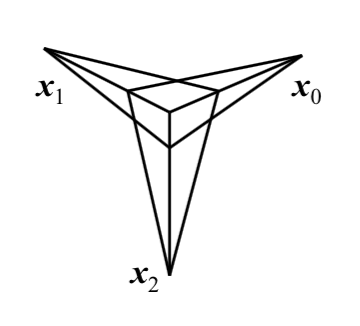
\includegraphics[width=0.4\textwidth]{figures/vanishing_points.png}
\end{center}
\caption{Visualisation of how the edges of a cuboid give rise to three orthogonal vanishing points: $x_0$, $x_1$, and $x_2$.} % TODO hur referera? Tagen från szeliski s. 330
\label{fig:vanishing_points}
\end{figure}

When $K$ had been obtained by either calibration method, the camera pose was estimated as described in \ref{camera-pose}, using the four image-world point correspondences given by the reference object.
The method EPnP was chosen initially, but much better results were achieved with a regular, iterative approach.

Once the camera pose was obtained, equation \ref{eq:projection1} could be used, meaning that any point in the world can be projected to a point in the image.
However, the reverse mapping was sought, i.e. the position of the package the world of the image coordinates of the bottom corners of the package.
This is not possible to do, unless something is known about the geometry of the scene.
Luckily, it is known that each lower corner shares $X$, and $Y$ coordinates with a top corner, which position is already known.
The image coordinates $(u,v)$ of a lower corner, and the world coordinates $(X,Y)$ of the corresponding upper corner ccould then be used to solve for the $Z$ coordinate of the lower corner. 
Equation \ref{eq:projection3} was transformed to the following over-determined system:
\begin{equation} \label{eq:constrained-projection}
\begin{pmatrix} up_{33}-p_{13} \\ vp_{33}-p_{23} \end{pmatrix} Z = 
\begin{pmatrix}
X(p_{11}-up_{31}) + Y(p_{12}-up_{32})+p_{14}-u \\
X(p_{21}-vp_{31}) + Y(p_{22}-vp_{32})+p_{24}-v
\end{pmatrix}
\end{equation}
This was solved as a least-squares problem using Single Value Decomposition (SVD).
Since two pairs of upper-lower corners which share $X$ and $Y$ coordinates were known, two least-squares solutions of $Z$ could be obtained.
The solution with the smallest error was chosen as $Z$.

\section{Evaluation}
To evaluate the performance of the method, a test dataset of 225 images of packages were taken.
Five different packages were in the dataset, with 45 images of each.
The packages in the test dataset are shown in figure \ref{fig:packages}. A blue plastic folder was placed under the reference object on packages 3-5 to add some contrast between the reference object and the white surfaces.
The images were taken with a Samsung Galaxy Edge S6 at 16 megapixels ($2988 \times 5312$ pixels) and then scaled down to $720 \times 1280$ pixels, to reduce computational time.
More about the hardware in section \ref{method:online_testing}.

\begin{figure}
	\centering
	\begin{subfigure}[b]{0.3\textwidth}
		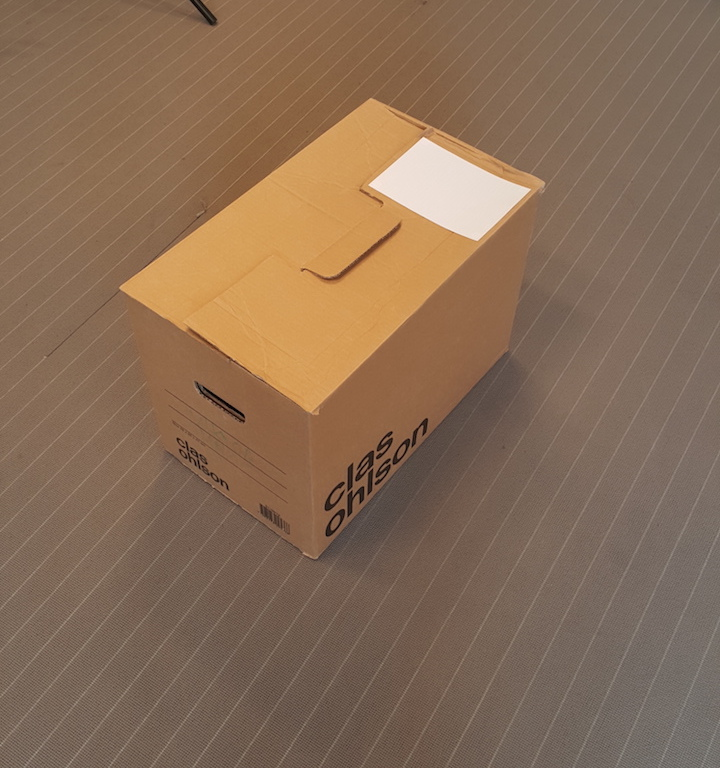
\includegraphics[width=\textwidth]{figures/package_1.jpg}
		\caption{}
		\label{fig:package_1}
	\end{subfigure}%
	~~~ %add desired spacing between images, e. g. ~, \quad, \qquad, \hfill etc.
	%(or a blank line to force the subfigure onto a new line)
	\begin{subfigure}[b]{0.3\textwidth}
		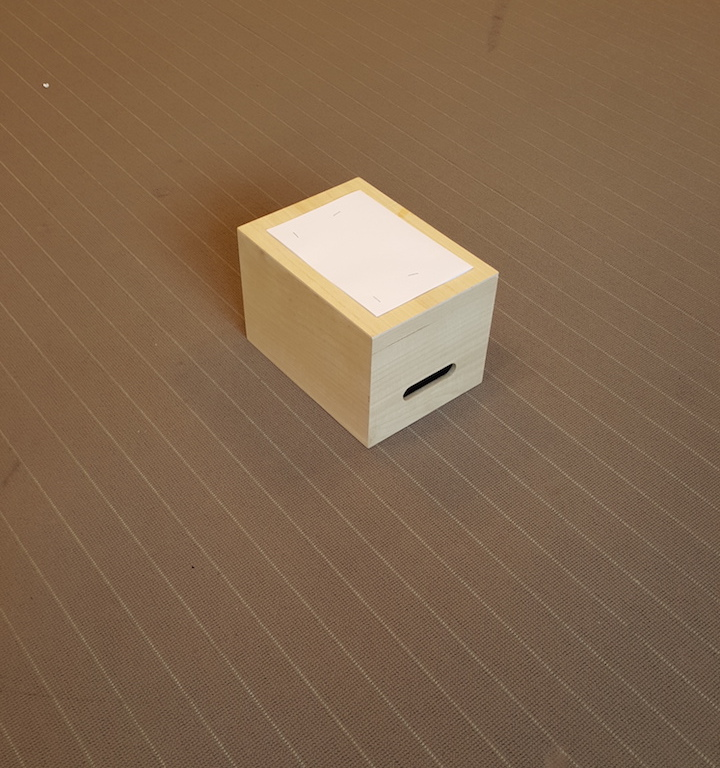
\includegraphics[width=\textwidth]{figures/package_2.jpg}
		\caption{}
		\label{fig:package_2}
	\end{subfigure}
	\vspace{3mm}\\
	\begin{subfigure}[b]{0.3\textwidth}
		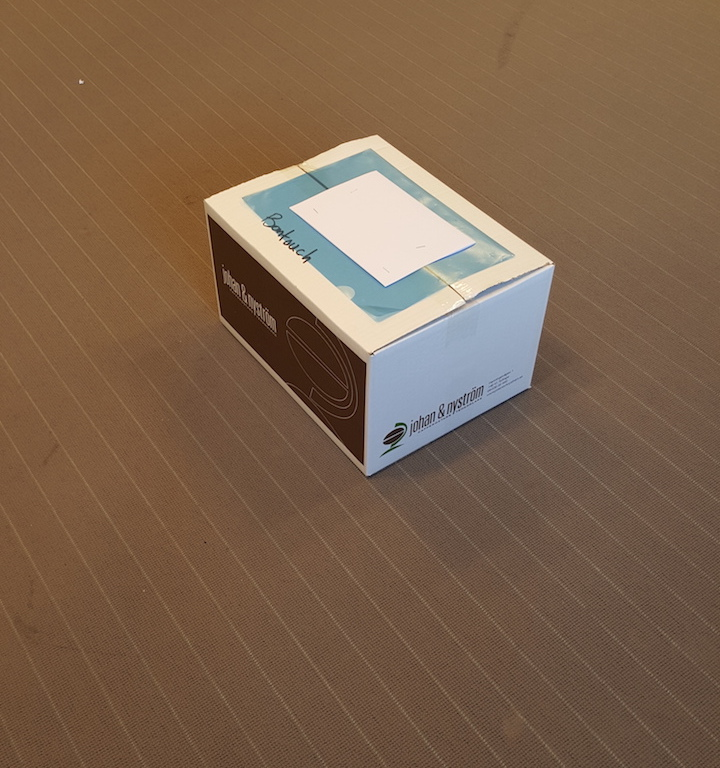
\includegraphics[width=\textwidth]{figures/package_3.jpg}
		\caption{}
		\label{fig:package_3}
	\end{subfigure}
	~~~
	\begin{subfigure}[b]{0.3\textwidth}
		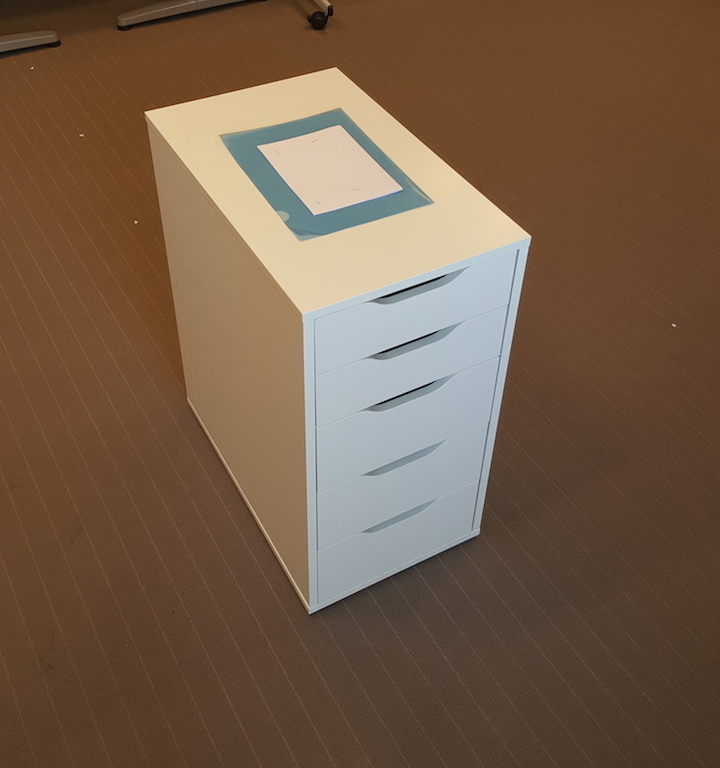
\includegraphics[width=\textwidth]{figures/package_4.jpg}
		\caption{}
		\label{fig:package_4}
	\end{subfigure}
	\vspace{3mm}\\
	\begin{subfigure}[b]{0.3\textwidth}
		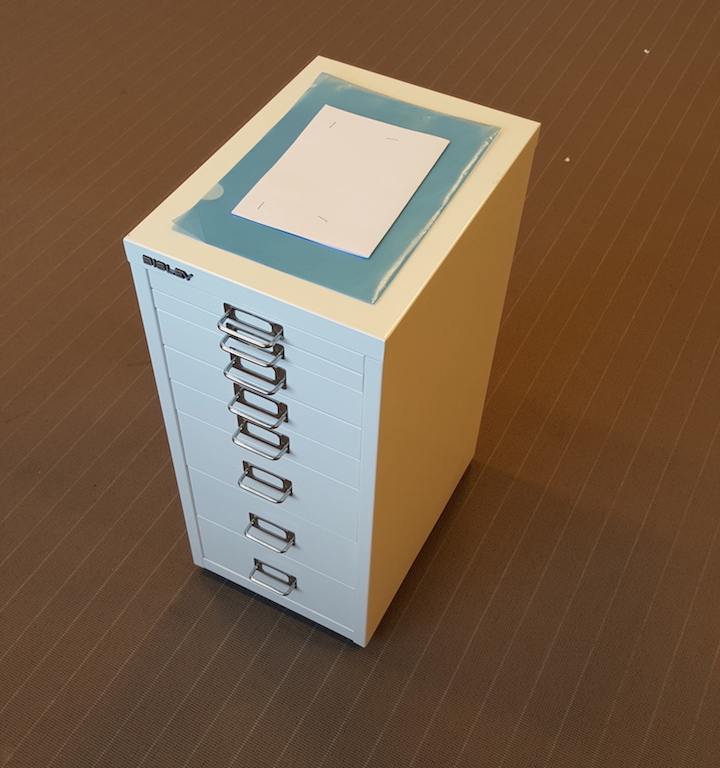
\includegraphics[width=\textwidth]{figures/package_5.jpg}
		\caption{}
		\label{fig:package_5}
	\end{subfigure}
	\caption[The packages in the test dataset]{The packages in the test dataset. (a) Package 1: A moving box ($580 \times 350 \times 405$ mm). (b) Package 2: A small wooden box ($260 \times 191 \times 177$ mm). (c) Package 3: A lightly textured cardboard box ($385 \times 295 \times 225$ mm). (d) Package 4: A white wooden filing cabinet ($580 \times 360 \times 690$ mm). (e) Package 5: A white metal filing cabinet ($383 \times 280 \times 605$ mm).}\label{fig:packages}
\end{figure}

The test dataset was constructed systematically with images observing the packages from different positions.
Three parameters were alternated: 
\begin{itemize}
	\item Distance to the centre of the package. 
			The used distances were 1, 1.5, and 2 metres.
	\item Height above the floor. 
			The used heights were 0.9, 1.2, and 1.5 metres for the first three packages, and 1.2, 1.5, and 1.8 metres for the latter two.
			The reason for the division is that the high height of the two latter packages made the viewing angle very small when viewing them from 0.9 metres above ground. The lowest height was removed for these packages and a higher one added.
	\item Rotation. 
			Five different angles were used.
			Two were frontal views of the package, in which only two faces of the package could be observed. One of the longer side, and one of the shorter side.
			One image was taken between the two sides, with a $45^\circ$ angle to both sides.
			The last two images view the package with a sharp angle, about $15^\circ$ to the long or short side, respectively.
			An example from each position is shown in figure \ref{fig:positions}.
\end{itemize}

\begin{figure}
	\centering
	\begin{subfigure}[b]{0.2\textwidth}
		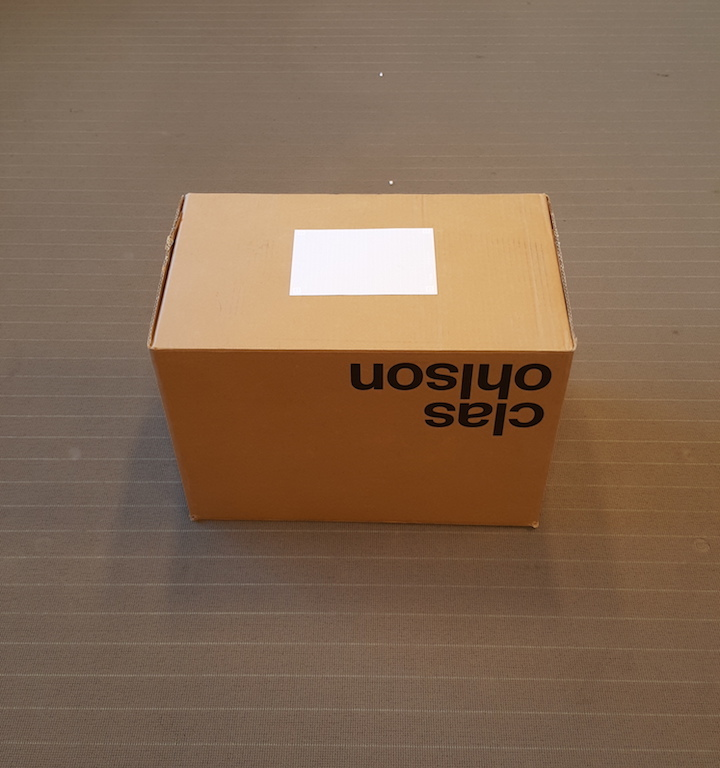
\includegraphics[width=\textwidth]{figures/angle_1.jpg}
		\label{fig:angle_1}
	\end{subfigure}
	~
	\begin{subfigure}[b]{0.2\textwidth}
		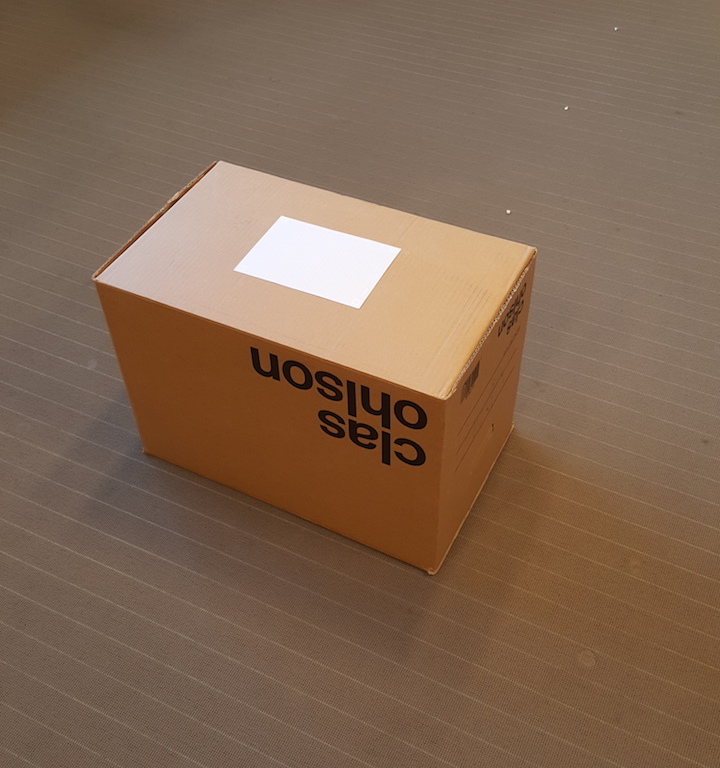
\includegraphics[width=\textwidth]{figures/angle_2.jpg}
		\label{fig:angle_2}
	\end{subfigure}
	~
	\begin{subfigure}[b]{0.2\textwidth}
		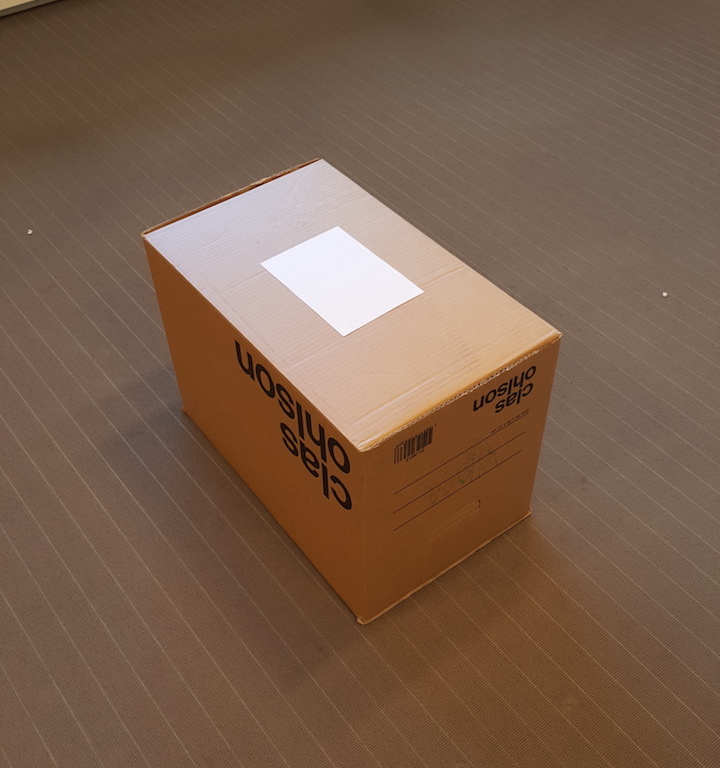
\includegraphics[width=\textwidth]{figures/angle_3.jpg}
		\label{fig:angle_3}
	\end{subfigure}
	
	\begin{subfigure}[b]{0.2\textwidth}
		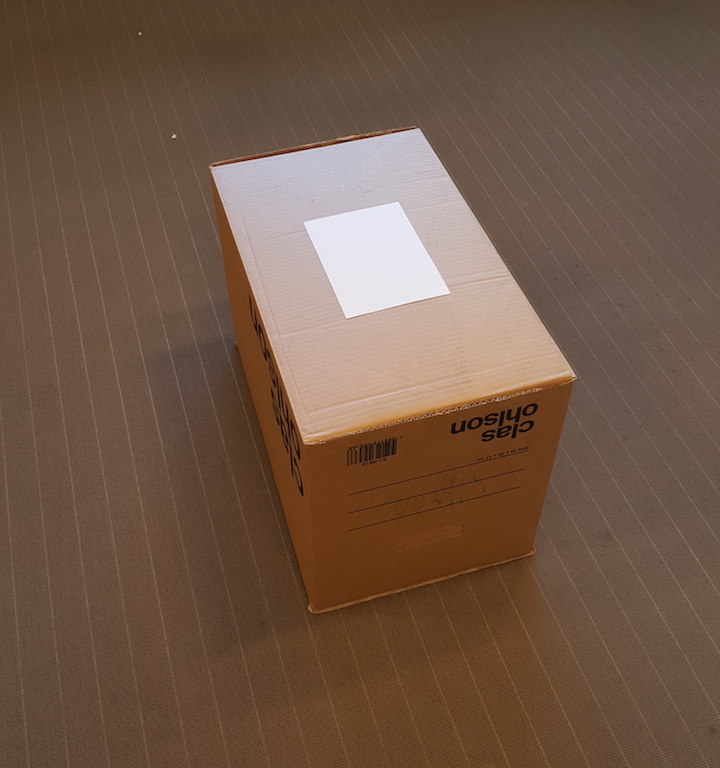
\includegraphics[width=\textwidth]{figures/angle_4.jpg}
		\label{fig:angle_4}
	\end{subfigure}
	~
	\begin{subfigure}[b]{0.2\textwidth}
		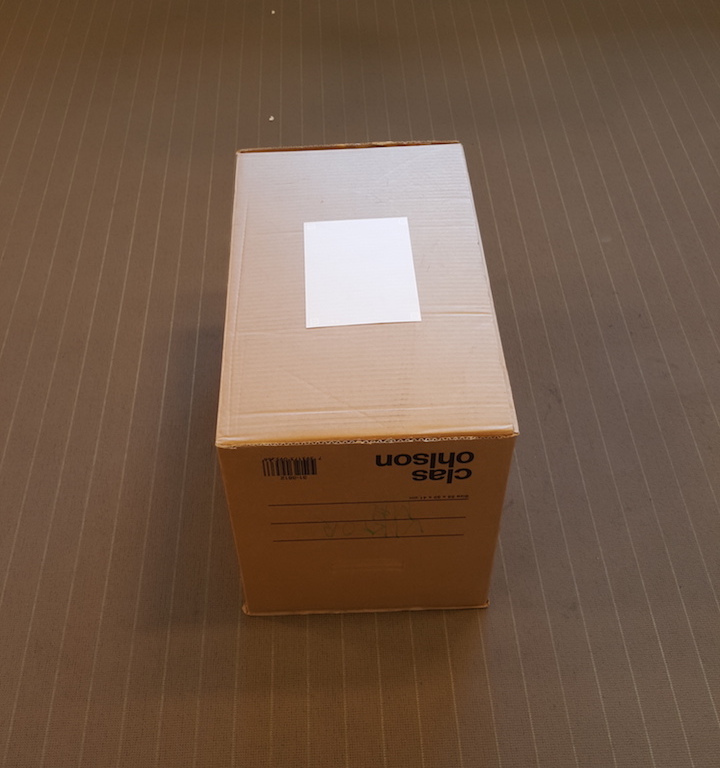
\includegraphics[width=\textwidth]{figures/angle_5.jpg}
		\label{fig:angle_5}
	\end{subfigure}
	\caption{Package 1 observed from the five different horizontal angles.}\label{fig:positions}
\end{figure}

\subsection{Benchmarking} \label{benchmarking}
A benchmarking program was made in order to measure the performance of the algorithm on the test dataset.
The detection algorithm and measuring algorithm were tested both in isolation, and combined, to show the performance of the individual pieces and of the whole system. 

The detection algorithm was tested by comparing the resulting corner points against ground truth positions of the reference object and package corners, which had been extracted manually in each image.

The measuring algorithm was tested by using the ground truth positions as input, and comparing the resulting measurements against the ground truth dimensions of the package.
Measurements were made with both calibration methods:, online vanishing point calibration, and offline calibration with Zhang's method. 

Finally, the overall ability of the system was tested by running the whole algorithm and comparing the result with the ground truth dimensions of the package. 

\subsection{Online testing} \label{method:online_testing}
A simple proof of concept Android application was made for online testing a the smartphone.
This was used to assert that it is feasible to run the algorithm on a smartphone.
Its purpose was also to determine if running the detection algorithm in real-time is feasible.

The app simply displays the camera feed and continuously feeds new frames to the measuring algorithm.
When the package or reference object is successfully detected, an overlay is drawn to outline their position on the screen.
If both the package and reference are found in the same frame, the dimensions of the package are calculated, and each dimension is drawn next to the appropriate edge.
The processing time for each frame is also displayed.
Screenshots of the application are shown in section \ref{results:online}.

The device used to run the test app is a Samsung Galaxy S6 Edge.
The S6 Edge was chosen because it currently tops benchmarks and tests, both regarding processing power and photo quality \cite{phone_performance_benchmark}\cite{phone_camera_benchmark}.
The S6 Edge was also used to capture the test images used for offline testing.










